% ============================================================================
%  forgethreads -- Presentación JCC 2026 (máx. 8 minutos)
%  Compilar:  pdflatex presentacion_jcc.tex  (dos pasadas)
%  Requiere:  fig1.png en la misma carpeta (Fig. 1 del paper)
% ============================================================================
\documentclass[aspectratio=169,10pt,xcolor=table]{beamer}

\usepackage[utf8]{inputenc}
\usepackage[T1]{fontenc}
\usepackage[spanish,es-noshorthands,es-nodecimaldot,es-notilde]{babel}
\usepackage[scaled=0.92]{helvet}
\usepackage{courier}
\renewcommand{\familydefault}{\sfdefault}
\usepackage{amsmath,amssymb}
\usepackage{booktabs}
\usepackage{listings}
\usepackage{tikz}
\usetikzlibrary{arrows.meta,positioning,calc,decorations.pathreplacing,3d,shapes.misc}
\usepackage{pgfplots}
\pgfplotsset{compat=1.16}

% ---------------------------------------------------------------------------
%  Tema estilo UCT (azul institucional + dorado)
% ---------------------------------------------------------------------------
\definecolor{uctazul}{RGB}{0,61,121}
\definecolor{uctazulclaro}{RGB}{0,104,178}
\definecolor{uctoro}{RGB}{242,169,0}
\definecolor{uctgris}{RGB}{90,90,90}
\definecolor{uctfondo}{RGB}{238,243,249}
\definecolor{acento}{RGB}{196,40,40}

\usetheme{default}
\setbeamertemplate{navigation symbols}{}
\setbeamercolor{structure}{fg=uctazul}
\setbeamercolor{normal text}{fg=black!85}
\setbeamercolor{alerted text}{fg=acento}
\setbeamercolor{block title}{bg=uctazul,fg=white}
\setbeamercolor{block body}{bg=uctfondo}
\setbeamerfont{frametitle}{size=\Large,series=\bfseries}
\setbeamertemplate{itemize item}{\color{uctoro}$\blacktriangleright$}
\setbeamertemplate{itemize subitem}{\color{uctazulclaro}\textbullet}
\setbeamertemplate{blocks}[rounded][shadow=false]

% Título de cada frame: barra azul + filete dorado
\setbeamercolor{frametitle}{bg=uctazul,fg=white}
\setbeamercolor{filete}{bg=uctoro}
\setbeamercolor{pie}{bg=uctazul,fg=white}
\setbeamercolor{pienum}{bg=uctazul,fg=uctoro}
\setbeamertemplate{frametitle}{%
  \nointerlineskip
  \begin{beamercolorbox}[wd=\paperwidth,ht=3.3ex,dp=1.5ex,leftskip=1.2em]{frametitle}%
    \usebeamerfont{frametitle}\insertframetitle
  \end{beamercolorbox}%
  \nointerlineskip
  \begin{beamercolorbox}[wd=\paperwidth,ht=0.45ex,dp=0pt]{filete}\end{beamercolorbox}%
  \vspace{1.2ex}%
}

% Pie de página
\setbeamertemplate{footline}{%
  \leavevmode\hbox{%
  \begin{beamercolorbox}[wd=.30\paperwidth,ht=2.4ex,dp=1ex,leftskip=1em]{pie}%
    \tiny Riquelme-Ávila, Rojas-Mora, Mardones-Arias
  \end{beamercolorbox}%
  \begin{beamercolorbox}[wd=.58\paperwidth,ht=2.4ex,dp=1ex,center]{pie}%
    \tiny CUDA y profundidad de parada en efectos olvidados max--min \;·\; JCC 2026
  \end{beamercolorbox}%
  \begin{beamercolorbox}[wd=.12\paperwidth,ht=2.4ex,dp=1ex,right,rightskip=1em]{pienum}%
    \tiny\bfseries\insertframenumber/\inserttotalframenumber
  \end{beamercolorbox}}%
}

% Código
\lstdefinestyle{cuda}{
  language=C++, basicstyle=\ttfamily\fontsize{6.6}{7.8}\selectfont, keywordstyle=\color{uctazul}\bfseries,
  commentstyle=\color{uctgris}\itshape, stringstyle=\color{acento},
  morekeywords={__hge,__hsub,__global__,__shared__,__syncthreads,__half,__hmin,__hgt,atomicAdd,extern},
  backgroundcolor=\color{uctfondo}, frame=single, rulecolor=\color{uctazul!40},
  xleftmargin=4pt, framexleftmargin=4pt, aboveskip=2pt, belowskip=2pt,
  showstringspaces=false, columns=fullflexible, keepspaces=true}

\newcommand{\ft}{\textbf{\color{uctazul}forgethreads}}
\newcommand{\fe}{\textbf{\color{uctgris}forgeffects}}
\newcommand{\cifra}[1]{{\color{uctazul}\bfseries #1}}

\title{Aceleración CUDA y regímenes empíricos de\\profundidad de parada en efectos olvidados max--min}
\author{Carlos Riquelme-Ávila \and Julio Rojas-Mora \and Elliott Mardones-Arias}
\institute{Universidad Católica de Temuco, Chile}
\date{Jornadas Chilenas de Computación (JCC) 2026}

\begin{document}
\unaccentedoperators

% ===========================================================================
% 1. Portada
% ===========================================================================
{
\setbeamertemplate{footline}{}
\begin{frame}[plain]
  \begin{tikzpicture}[remember picture,overlay]
    \fill[uctazul] (current page.north west) rectangle ([yshift=-0.58\paperheight]current page.north east);
    \fill[uctoro]  ([yshift=-0.58\paperheight]current page.north west) rectangle ([yshift=-0.60\paperheight]current page.north east);
    % Para usar el logo institucional, descomentar y ajustar la ruta:
    % \node[anchor=north east] at ([xshift=-6mm,yshift=-5mm]current page.north east)
    %      {\includegraphics[height=1.3cm]{logo_uct.png}};
    \node[anchor=west,text width=0.86\paperwidth,align=left,text=white]
      at ([xshift=8mm,yshift=-0.30\paperheight]current page.north west)
      {{\Large\bfseries\inserttitle}\\[3mm]
       {\normalsize\color{uctoro} forgethreads: max--min con memoria cuadrática en GPU}};
    \node[anchor=north west,text width=0.86\paperwidth,align=left]
      at ([xshift=8mm,yshift=-0.65\paperheight]current page.north west)
      {{\bfseries Carlos Riquelme-Ávila \quad Julio Rojas-Mora \quad Elliott Mardones-Arias}\\[1.5mm]
       {\small\color{uctgris} Universidad Católica de Temuco, Chile}\\[3mm]
       {\small\color{uctazul}\insertdate}};
  \end{tikzpicture}
\end{frame}
}

% ===========================================================================
% 2. Problema
% ===========================================================================
\begin{frame}{El problema: efectos olvidados y el orden de detención}
\centering
\begin{tikzpicture}[font=\small,
  nd/.style={circle,draw=uctazul,very thick,fill=uctfondo,minimum size=7mm,font=\small\bfseries}]
  % grafo
  \node[nd] (a) at (0,0) {$i$};
  \node[nd] (b) at (1.6,0.9) {$k$};
  \node[nd] (c) at (3.2,0) {$j$};
  \draw[-{Stealth},thick,uctazul] (a) -- node[above left,font=\scriptsize]{0.9} (b);
  \draw[-{Stealth},thick,uctazul] (b) -- node[above right,font=\scriptsize]{0.7} (c);
  \draw[-{Stealth},thick,dashed,acento] (a) to[bend right=30] node[below,font=\scriptsize]{efecto olvidado: 0.7} (c);
  \node[font=\scriptsize,text=uctgris] at (1.6,-1.35) {no está en $E$; aparece por un camino};
  % cadena de órdenes
  \begin{scope}[shift={(5.2,0.2)},
    st/.style={draw=uctazul,thick,rounded corners,fill=uctfondo,minimum width=1.0cm,minimum height=0.7cm,font=\scriptsize}]
    \node[st] (e1) at (0,0) {$E^{(1)}$};
    \node[st] (e2) at (1.35,0) {$E^{(2)}$};
    \node (dt) at (2.5,0) {$\cdots$};
    \node[st,fill=uctoro!35,draw=uctoro!80!black] (en) at (3.65,0) {$E^{(\eta_0)}$};
    \node[st,draw=gray,fill=gray!10] (ef) at (5.1,0) {$E^{(\eta_0+1)}$};
    \foreach \u/\v in {e1/e2,e2/dt,dt/en,en/ef} \draw[-{Stealth},thick] (\u) -- (\v);
    % barras q_r
    \foreach \x/\h in {0/0.35,1.35/0.8,2.2/0.6,2.8/0.35,3.65/0.15}{
      \fill[uctazul] (\x-0.12,-1.45) rectangle (\x+0.12,-1.45+\h);}
    \draw (-0.5,-1.45) -- (5.6,-1.45);
    \node[font=\scriptsize,anchor=east] at (-0.55,-1.2) {$q_r$};
    \node[font=\scriptsize,text=acento] at (5.1,-1.25) {$q=0$};
    \node[font=\scriptsize,text=acento] at (5.1,-0.65) {parar};
  \end{scope}
\end{tikzpicture}

\vspace{6mm}
\begin{columns}[T]
\column{0.46\textwidth}
\begin{block}{Ingeniería}
\small Cada orden cuesta $\mathcal{O}(N^3)$. ¿Cómo escalar?
\end{block}
\column{0.46\textwidth}
\begin{block}{Ciencia}
\small ¿De qué depende el orden de detención $\eta_0$?
\end{block}
\end{columns}
\end{frame}

% ===========================================================================
% 3. Composición max-min
% ===========================================================================
\begin{frame}{La composición max--min}
\begin{columns}[c]
\column{0.42\textwidth}
\centering
\[
  E^{(r+1)}_{ij} = \max_{k}\ \min\big(E^{(r)}_{ik},E_{kj}\big)
\]
\vspace{2mm}
\begin{tikzpicture}[font=\small]
  \node[draw=uctgris,rounded corners,fill=gray!8,minimum width=2.3cm] (g) at (0,0) {$\sum_k a\cdot b$};
  \node[draw=uctazul,rounded corners,fill=uctfondo,minimum width=2.3cm] (m) at (0,-1.3) {$\max_k \min(a,b)$};
  \draw[-{Stealth},thick] (g) -- (m);
  \node[font=\scriptsize,anchor=west] at (1.3,0) {producto de matrices};
  \node[font=\scriptsize,anchor=west] at (1.3,-1.3) {max--min};
\end{tikzpicture}

\vspace{3mm}
{\small Es un \textbf{GEMM} con otras operaciones.}

\column{0.56\textwidth}
\centering
\begin{tikzpicture}[font=\scriptsize]
  \def\w{0.95}
  \node[anchor=east] at (-0.1,1.6) {fila $i$ de $E^{(r)}$};
  \node[anchor=east] at (-0.1,0.9) {columna $j$ de $E$};
  \node[anchor=east] at (-0.1,0.2) {$\min$};
  \foreach \k/\a/\b/\m in {0/0.9/0.7/0.7,1/0.3/0.8/0.3,2/1.0/0.2/0.2,3/0.4/0.6/0.4}{
    \node[draw=uctazul,fill=uctfondo,minimum width=0.8cm] at (\k*\w+0.4,1.6) {\a};
    \node[draw=uctazul,fill=uctfondo,minimum width=0.8cm] at (\k*\w+0.4,0.9) {\b};
    \node[draw=gray,minimum width=0.8cm] at (\k*\w+0.4,0.2) {\m};
    \node[font=\tiny,text=uctgris] at (\k*\w+0.4,2.1) {$k=\k$};
  }
  \node[draw=uctoro!80!black,fill=uctoro!40,thick,minimum width=0.8cm] at (0.4,0.2) {0.7};
  \draw[-{Stealth},thick,uctoro!80!black] (0.4,-0.15) -- (0.4,-0.6);
  \node[anchor=north] at (1.8,-0.6) {$\max=0.7 \Rightarrow E^{(r+1)}_{ij}=0.7$};
\end{tikzpicture}

\vspace{4mm}
{\small Arista más débil ($\min$), mejor camino ($\max$).\\
$N^2$ celdas $\times$ $N$ candidatos $=$ \cifra{$\mathcal{O}(N^3)$} por orden.}
\end{columns}
\end{frame}

% ===========================================================================
% 4. Arquitectura
% ===========================================================================
\begin{frame}{Arquitectura de forgethreads}
\centering
\vspace{3mm}
\begin{tikzpicture}[font=\small,
  lay/.style={draw=uctazul,thick,rounded corners,fill=uctfondo,minimum height=1.3cm,text width=3.1cm,align=center},
  gpu/.style={draw=uctoro!80!black,thick,rounded corners,fill=uctoro!18,minimum height=1.3cm,text width=3.1cm,align=center}]
  \node[lay] (py) at (0,0) {\textbf{Python}\\[-0.5mm]{\scriptsize TensorFlow / NumPy}};
  \node[lay] (bind) at (5.1,0) {\textbf{Bindings C++}\\[-0.5mm]{\scriptsize una llamada}};
  \node[gpu] (eng) at (10.2,0) {\textbf{Motor CUDA}\\[-0.5mm]{\scriptsize órdenes + kernel}};
  \node[draw=uctoro!80!black,dashed,thick,rounded corners,minimum width=13.6cm,minimum height=1.05cm,anchor=north] (mem) at (5.1,-1.3) {};
  \node[anchor=west,font=\scriptsize\bfseries,text=uctoro!80!black] at (mem.west) {\; Memoria GPU};
  \node[font=\scriptsize] at (6.6,-1.83) {$E$,\; $E^{(r)}$,\; $E^{(r+1)}$,\; $\kappa$,\; $q_r$ \quad $\mathcal{O}(N^2)$};
  \draw[-{Stealth},very thick,uctazul] ([yshift=2mm]py.east) -- node[above,font=\scriptsize]{DLPack} ([yshift=2mm]bind.west);
  \draw[{Stealth}-,very thick,uctazul] ([yshift=-2mm]py.east) -- node[below,font=\scriptsize]{resultados} ([yshift=-2mm]bind.west);
  \draw[-{Stealth},very thick,uctazul] (bind) -- (eng);
  \draw[{Stealth}-{Stealth},thick,uctoro!80!black] (py.south) -- ++(0,-0.45);
  \draw[{Stealth}-{Stealth},thick,uctoro!80!black] (eng.south) -- ++(0,-0.45);
  \node[font=\scriptsize,text=uctoro!80!black,anchor=west] at (0.15,-0.95) {\textbf{zero-copy}};
\end{tikzpicture}

\vspace{8mm}
{\small Los tensores se comparten por puntero: \textbf{sin copias} host--GPU.\\
Se itera hasta $q_r=0$ y se devuelven los efectos, $q_r$ y $\eta_0$.}
\end{frame}

% ===========================================================================
% 5. Kernel
% ===========================================================================
\begin{frame}{Kernel: tiling estilo GEMM + conteo}
\begin{columns}[c]
\column{0.52\textwidth}
\centering
\begin{tikzpicture}[font=\scriptsize,scale=1.0]
  \draw[uctazul!60,thick] (2.1,2.3) rectangle (4.5,3.3);
  \fill[uctazul!35] (3.0,2.3) rectangle (3.6,3.3);
  \node at (3.3,3.55) {$E$};
  \draw[uctazul!60,thick] (0,0) rectangle (1.6,2.0);
  \fill[uctazul!35] (0,0.8) rectangle (1.6,1.4);
  \node at (0.8,-0.25) {$E^{(r)}$};
  \draw[uctoro!80!black,thick] (2.1,0) rectangle (4.5,2.0);
  \fill[uctoro!40] (3.0,0.8) rectangle (3.6,1.4);
  \draw[step=0.15,uctoro!80!black,very thin] (3.0,0.8) grid (3.6,1.4);
  \node at (3.3,-0.25) {$E^{(r+1)}$};
  \draw[-{Stealth},thick] (3.6,1.1) -- (4.9,1.1) node[right,align=left]{1 hilo =\\$8\times8$ celdas};
  \node[draw=uctazul,rounded corners,fill=uctfondo,align=center,font=\tiny] at (0.8,2.8) {tiles $64\times64$ en\\memoria compartida};
\end{tikzpicture}

\column{0.46\textwidth}
\small
\renewcommand{\arraystretch}{1.35}
\begin{tabular}{@{}l c c@{}}
\toprule
 & GEMM & max--min \\
\midrule
operación & $a\cdot b$ & $\min$ \\
acumulador & $+$ & $\max$ \\
epílogo & $\alpha AB+\beta C$ & \cellcolor{uctoro!30}\textbf{¿$\Delta\ge\epsilon$? $\to q_r$\,+1} \\
\bottomrule
\end{tabular}

\vspace{5mm}
\begin{block}{Lo nuevo}
\small $q_r$ se cuenta \textbf{en la misma pasada}, con un contador atómico.
\end{block}
\end{columns}
\end{frame}

% ===========================================================================
% 6. Rendimiento y límites
% ===========================================================================
\begin{frame}{Rendimiento y límites en una RTX 4090}
\begin{columns}[T]
\column{0.58\textwidth}
\centering
\begin{tikzpicture}
\begin{axis}[
  width=8.4cm,height=6.1cm,
  ymode=log, xlabel={Nodos $N$}, ylabel={Tiempo (ms)},
  xtick={150,300,600,900,1200}, xticklabel style={font=\scriptsize,/pgf/number format/1000 sep={}},
  yticklabel style={font=\scriptsize}, label style={font=\small},
  legend style={font=\tiny,at={(0.02,0.98)},anchor=north west,draw=none,fill=white,fill opacity=0.85,text opacity=1},
  legend cell align=left,
  grid=major, grid style={gray!20}, ymin=0.1, ymax=2000]
  \addplot[mark=square*,thick,color=uctgris] coordinates
    {(150,8.050) (300,8.885) (600,15.578) (700,19.778) (900,40.612) (1200,57.175)};
  \addlegendentry{forgeffects (TensorFlow)}
  \addplot[mark=triangle*,thick,color=acento!80] coordinates
    {(150,0.176) (300,0.958) (600,6.333) (700,9.624) (900,24.406) (1200,75.165)};
  \addlegendentry{v1: bloque por celda}
  \addplot[mark=*,thick,color=uctazulclaro] coordinates
    {(150,0.183) (300,0.226) (600,0.753) (700,1.019) (900,1.874) (1200,4.465)};
  \addlegendentry{v2: tiles $32\times32$}
  \addplot[mark=diamond*,mark size=2.6pt,thick,color=uctoro!85!black] coordinates
    {(150,0.324) (300,0.457) (600,1.015) (700,1.156) (900,1.717) (1200,4.075)};
  \addlegendentry{v4: tiling 2D $64\times64$}
\end{axis}
\end{tikzpicture}

{\tiny \texttt{float16}, 3 órdenes, media de 10 ejecuciones.}

\column{0.40\textwidth}
\centering
{\small\bfseries Speedup frente a forgeffects}\\[2mm]
\begin{tikzpicture}[font=\scriptsize]
  \fill[uctazulclaro] (0,0.6) rectangle (3.2,0.95); \node[anchor=west,text=white,font=\scriptsize\bfseries] at (0.05,0.775) {v2: 12.8--44$\times$};
  \fill[uctoro!85!black] (0,0) rectangle (1.8,0.35); \node[anchor=west,text=white,font=\scriptsize\bfseries] at (0.05,0.175) {v4: 14--25$\times$};
\end{tikzpicture}

\vspace{6mm}
{\small\bfseries Tamaño máximo (24\,GB)}\\[2mm]
\begin{tikzpicture}[font=\scriptsize]
  % escala log: x = 1.6*(log10 N - 3)
  \fill[uctgris] (0,0.6) rectangle (0.127,0.95);
  \node[anchor=west] at (0.2,0.775) {forgeffects: 1\,200 \alert{(OOM en 1\,300)}};
  \fill[uctazul] (0,0) rectangle (2.41,0.35);
  \node[anchor=west,text=white,font=\scriptsize\bfseries] at (0.05,0.175) {forgethreads: 32\,000};
  \draw[thin,gray] (0,-0.15) -- (2.9,-0.15);
  \foreach \x/\l in {0/1k,1.6/10k,2.41/32k}{\draw (\x,-0.1)--(\x,-0.2) node[below,font=\tiny]{\l};}
\end{tikzpicture}

\vspace{5mm}
{\footnotesize forgeffects es útil, pero su memoria crece como $N^3$.}
\end{columns}
\end{frame}

% ===========================================================================
% 7. Recurso finito
% ===========================================================================
\begin{frame}{Profundidad de parada: un recurso finito}
\begin{columns}[c]
\column{0.40\textwidth}
\[ q_r=\#\{(i,j):\Delta^{(r)}_{ij}>\epsilon\} \]
\[ \eta_0=\max\{r:q_r>0\} \]
\vspace{2mm}
\begin{block}{Con $\epsilon=1/2$}
\small Cada par se descubre \textbf{una sola vez}: dos saltos $>\tfrac12$ superarían 1.\\[1mm]
$\Rightarrow \sum_r q_r \le N^2$
\end{block}
\vspace{2mm}
{\small $\eta_0$ = orden en que se gasta el \textbf{último} par.}

\column{0.58\textwidth}
\centering
\begin{tikzpicture}[font=\scriptsize]
  % rejilla: color = orden de descubrimiento (esquema)
  \def\ord{{1,2,1,3,2,4,1,2, 2,1,3,2,4,1,2,3, 1,3,1,2,1,2,5,1, 3,2,2,1,3,1,2,4, 2,4,1,3,1,2,1,2, 4,1,2,1,2,1,3,6, 1,2,5,2,3,2,1,2, 2,3,1,4,2,3,2,1}}
  \foreach \i in {0,...,7}{\foreach \j in {0,...,7}{
    \pgfmathtruncatemacro{\o}{\ord[\i*8+\j]}
    \pgfmathtruncatemacro{\c}{\o*17}
    \ifnum\o=6 \fill[acento] (\j*0.36,-\i*0.36) rectangle ++(0.34,-0.34);
    \else \fill[uctazul!\c!white] (\j*0.36,-\i*0.36) rectangle ++(0.34,-0.34);\fi
  }}
  \node[anchor=south] at (1.44,0.05) {cada par $(i,j)$: el orden en que se descubre};
  % histograma
  \begin{scope}[shift={(3.4,-2.9)}]
    \foreach \r/\h in {1/2.0,2/1.85,3/0.9,4/0.6,5/0.25,6/0.12}{
      \pgfmathtruncatemacro{\c}{\r*17}
      \ifnum\r=6 \fill[acento] (\r*0.32,0) rectangle ++(0.24,\h);
      \else \fill[uctazul!\c!white] (\r*0.32,0) rectangle ++(0.24,\h);\fi
      \node[below,font=\tiny] at (\r*0.32+0.12,0) {\r};
    }
    \draw (0.2,0) -- (2.3,0);
    \node[below,font=\tiny] at (1.25,-0.25) {orden $r$};
    \node[font=\tiny,anchor=south] at (1.25,2.05) {$q_r$};
    \draw[-{Stealth},acento,thick] (2.25,0.8) node[above,font=\tiny]{$\eta_0$} -- (2.05,0.18);
  \end{scope}
\end{tikzpicture}

{\tiny (esquema ilustrativo)}
\end{columns}
\end{frame}

% ===========================================================================
% 8. Diseño
% ===========================================================================
\begin{frame}{Diseño: dos bloques, un parámetro $c$}
\begin{columns}[c]
\column{0.38\textwidth}
\centering
\begin{tikzpicture}[font=\small]
  \fill[uctazul!25] (0,1.6) rectangle (1.6,3.2);
  \fill[uctazul!12] (1.6,1.6) rectangle (3.2,3.2);
  \fill[gray!10]    (0,0) rectangle (1.6,1.6);
  \fill[uctoro!35]  (1.6,0) rectangle (3.2,1.6);
  \draw[thick] (0,0) rectangle (3.2,3.2);
  \draw (1.6,0) -- (1.6,3.2) (0,1.6) -- (3.2,1.6);
  \node at (0.8,2.4) {$E_{\mathcal{NN}}$};
  \node at (2.4,2.4) {$E_{\mathcal{NM}}$};
  \node at (0.8,0.8) {$0$};
  \node at (2.4,0.8) {$E_{\mathcal{MM}}$};
  \node[font=\scriptsize,above] at (0.8,3.2) {$\mathcal{N}$};
  \node[font=\scriptsize,above] at (2.4,3.2) {$\mathcal{M}$};
  \node[font=\scriptsize] at (1.6,-0.4) {solo $\mathcal{N}\to\mathcal{M}$ · binaria};
\end{tikzpicture}

\column{0.60\textwidth}
\centering
{\small $c$ = grado de salida esperado por fila}\\[3mm]
\begin{tikzpicture}[font=\small]
  % fila de M
  \node[anchor=east] at (0,1.2) {fila de $\mathcal{M}$};
  \fill[uctoro!70] (0.2,1.0) rectangle (4.2,1.4);
  \node[font=\scriptsize] at (2.2,1.2) {todo a $\mathcal{M}$: $d_{\mathcal{MM}}=c$};
  % fila de N
  \node[anchor=east] at (0,0.3) {fila de $\mathcal{N}$};
  \fill[uctazul!50] (0.2,0.1) rectangle (2.2,0.5);
  \fill[uctazul!20] (2.2,0.1) rectangle (4.2,0.5);
  \node[font=\scriptsize] at (1.2,0.3) {$d_{\mathcal{NN}}\approx c/2$};
  \node[font=\scriptsize] at (3.2,0.3) {$d_{\mathcal{NM}}\approx c/2$};
\end{tikzpicture}

\vspace{4mm}
{\small Cada bloque llega a \textbf{grado 1} en un $c$ distinto:}\\[1mm]
\begin{tikzpicture}[font=\scriptsize]
  \draw[-{Stealth},thick] (0,0) -- (6.0,0) node[right]{$c$};
  \foreach \x/\l in {0.3/{1/8},1.8/1,3.4/2,4.4/3,5.6/50}{\draw (\x,0.08)--(\x,-0.08) node[below]{$\l$};}
  \fill[uctoro!80!black] (1.8,0.25) circle (2.5pt) node[above,text=uctoro!80!black]{bloque $\mathcal{M}$};
  \fill[uctazul] (3.4,0.25) circle (2.5pt) node[above,text=uctazul]{bloque $\mathcal{N}$};
\end{tikzpicture}

\vspace{3mm}
{\footnotesize 7 tamaños ($n\le10\,000$) $\times$ 19 valores de $c$ $\times$ 20 réplicas = \cifra{2\,640 grafos}}
\end{columns}
\end{frame}

% ===========================================================================
% 10. Perfil
% ===========================================================================
\begin{frame}{Resultado: un perfil de dos ventanas}
\centering
\begin{tikzpicture}
  \node[inner sep=0] (f) {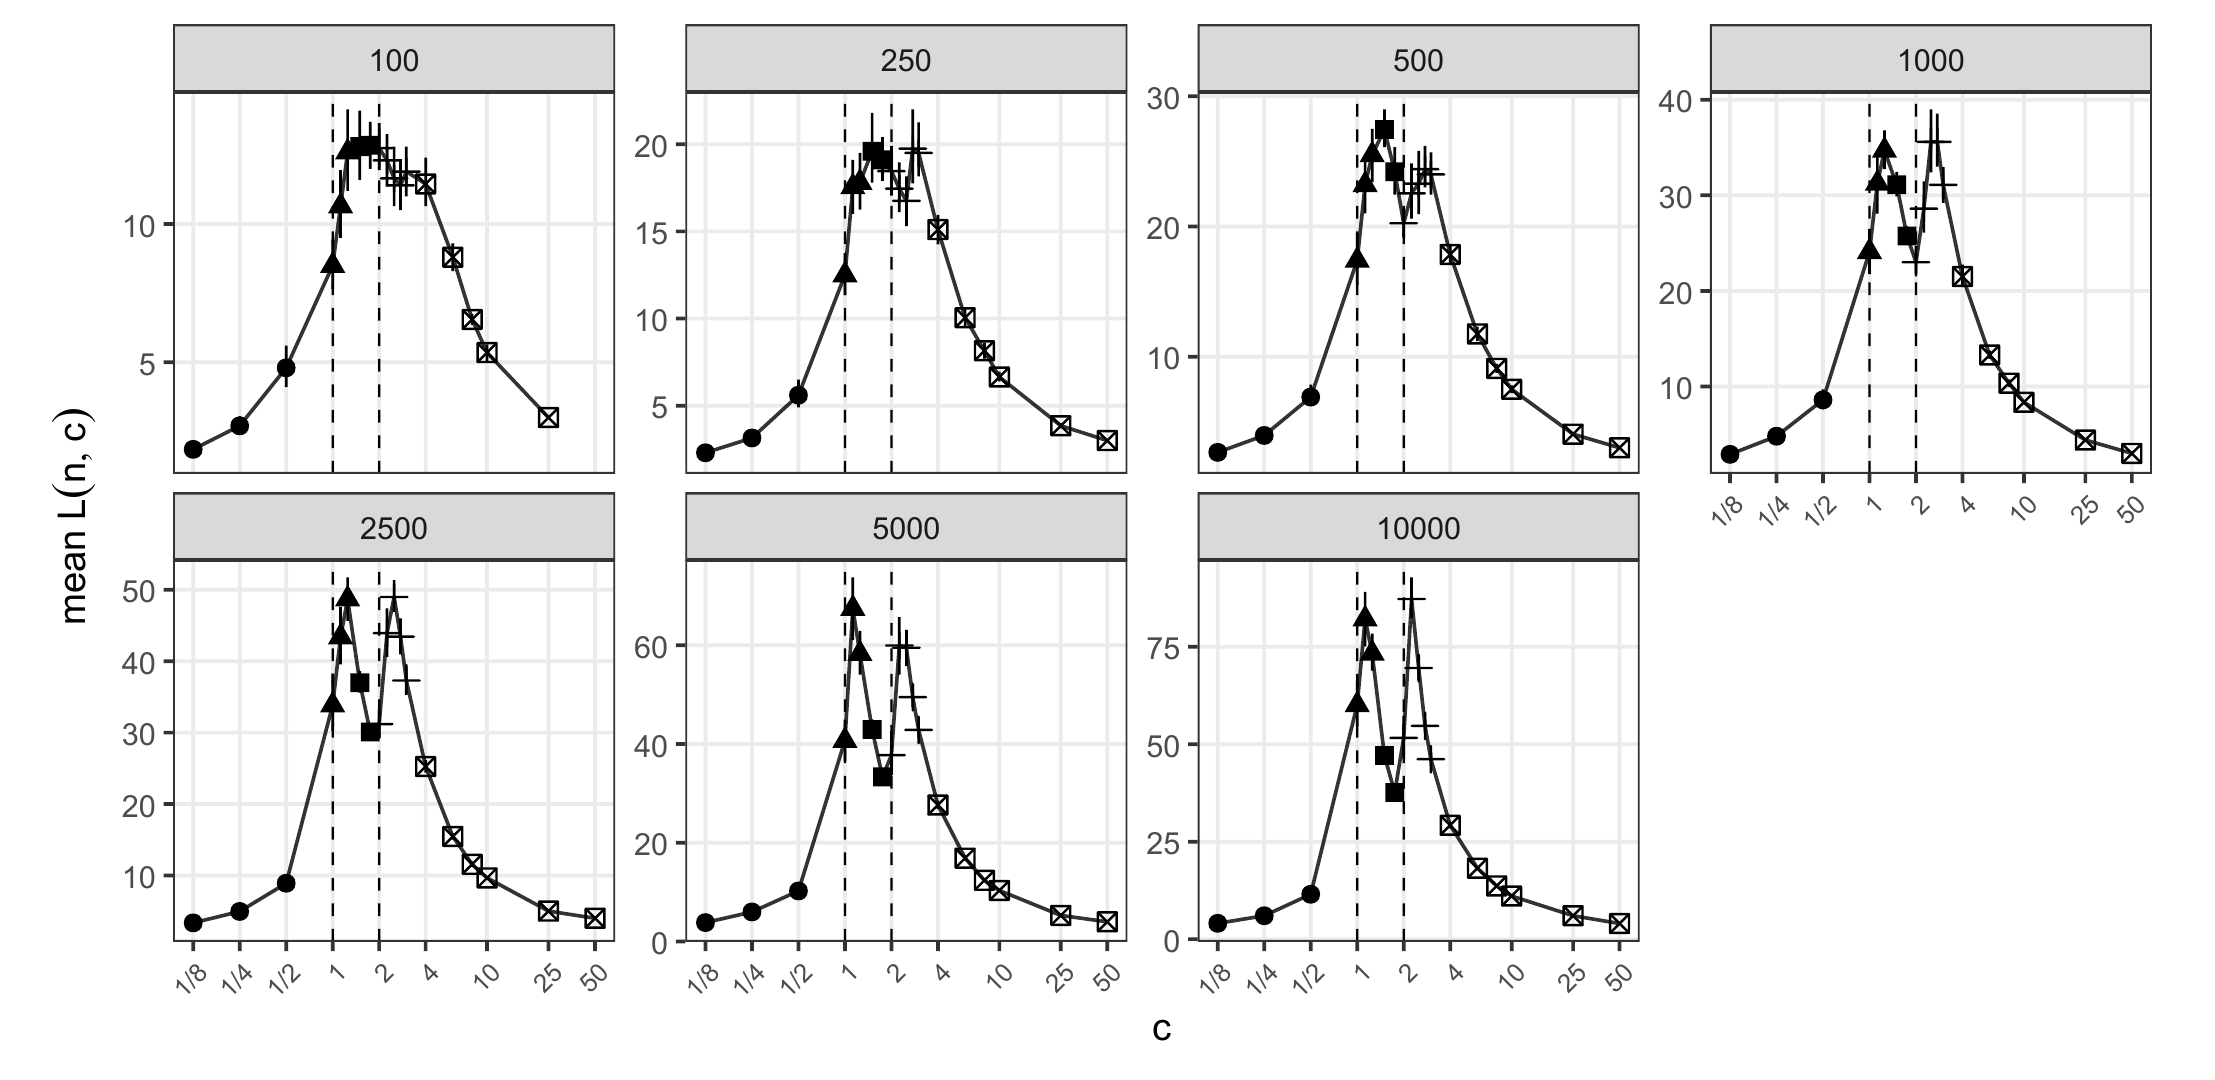
\includegraphics[width=0.86\textwidth]{fig1.png}};
  \node[anchor=south east,align=left,font=\scriptsize,inner sep=2pt]
    at ([xshift=-2mm,yshift=10mm]f.south east)
    {\textbullet\ baja conectividad\\
     $\blacktriangle$\ ventana $\mathcal{M}$\\
     $\blacksquare$\ valle\\
     $+$\ ventana $\mathcal{N}$\\
     $\boxtimes$\ atajos};
\end{tikzpicture}\\[1mm]
{\small Más conexiones \alert{no} implican más órdenes: \textbf{bajo $\to$ pico $\to$ valle $\to$ pico $\to$ caída}.}\\
{\tiny Un panel por tamaño $n$. Barras: intervalo de confianza 95\,\% (bootstrap). Líneas punteadas: $c=1$ y $c=2$.}
\end{frame}

% ===========================================================================
% 9. Regímenes
% ===========================================================================
\begin{frame}{Cinco regímenes}
\centering
\begin{tikzpicture}[x=1.15cm,font=\scriptsize]
  \def\xa{0}\def\xb{3}\def\xc{3.32}\def\xd{4}\def\xe{4.585}\def\xf{8.64}
  \fill[gray!18]    (\xa,0) rectangle (\xb,0.55);
  \fill[uctoro!80]  (\xb,0) rectangle (\xc,0.55);
  \fill[uctazul!15] (\xc,0) rectangle (\xd,0.55);
  \fill[uctazul!70] (\xd,0) rectangle (\xe,0.55);
  \fill[acento!18]  (\xe,0) rectangle (\xf,0.55);
  \draw[-{Stealth},thick] (\xa,0) -- (\xf+0.3,0) node[right]{$c$};
  \foreach \x/\l in {0/{1/8},1/{1/4},2/{1/2},3/1,4/2,4.585/3,6/8,8.64/50}{
    \draw (\x,0.06)--(\x,-0.08) node[below]{$\l$};}
  % barras de profundidad media sobre cada régimen
  \foreach \xl/\xr/\h/\v in {0/3/0.25/4.97, 3/3.32/1.74/34.87, 3.32/4/1.45/28.99, 4/4.585/1.68/33.64, 4.585/8.64/0.52/10.38}{
    \fill[black!65] ({(\xl+\xr)/2-0.12},0.75) rectangle ({(\xl+\xr)/2+0.12},0.75+\h);
    \node[above,font=\tiny] at ({(\xl+\xr)/2},0.75+\h) {\v};
  }
  \node[anchor=west,font=\tiny,text=uctgris] at (5.2,2.2) {barra: $\bar L=\eta_0$ medio};
  % etiquetas
  \node[align=center] at (1.5,-0.75) {baja\\conectividad};
  \node[align=center,text=uctoro!80!black] at (3.05,-0.75) {\textbf{ventana}\\$\mathcal{M}$};
  \node[align=center] at (3.75,-0.75) {valle};
  \node[align=center,text=uctazul] at (4.4,-0.75) {\textbf{ventana}\\$\mathcal{N}$};
  \node[align=center] at (6.6,-0.75) {atajos};
\end{tikzpicture}

\vspace{4mm}
\footnotesize
\renewcommand{\arraystretch}{1.2}
\begin{tabular}{@{}ll@{}}
\textbf{Baja conectividad} & cadenas cortas: se agotan pronto \\
\textbf{\color{uctoro!80!black}Ventana $\mathcal{M}$} & $\mathcal{M}$ en su umbral: cadenas largas y frágiles \\
\textbf{Valle} & $\mathcal{M}$ ya tiene atajos; $\mathcal{N}$ aún no llega \\
\textbf{\color{uctazul}Ventana $\mathcal{N}$} & $\mathcal{N}$ en su umbral \\
\textbf{Atajos} & muchos caminos cortos: todo se descubre temprano \\
\end{tabular}
\end{frame}

% ===========================================================================
% 11. Tamaño
% ===========================================================================
\begin{frame}{Las dos ventanas se marcan más al crecer $n$}
\begin{columns}[T]
\column{0.50\textwidth}
\centering
{\small\bfseries Ventana menos valle}\\[1mm]
\begin{tikzpicture}
\begin{axis}[width=7.0cm,height=4.8cm, xmode=log, log basis x=10,
  xtick={100,250,500,1000,2500,5000,10000},
  xticklabels={100,250,500,1k,2.5k,5k,10k},
  xticklabel style={font=\scriptsize}, yticklabel style={font=\scriptsize},
  xlabel={$n$}, ylabel={órdenes}, label style={font=\small},
  legend style={font=\scriptsize,at={(0.03,0.97)},anchor=north west,draw=none},
  grid=major, grid style={gray!20}]
  \fill[uctfondo] (axis cs:2000,-8) rectangle (axis cs:12500,32);
  \addplot[uctoro!85!black,thick,mark=triangle*,error bars/.cd,y dir=both,y explicit]
   coordinates {(100,-2.8) +- (0,1.2) (250,-4.6) +- (0,1.3) (500,-2.5) +- (0,2.05)
     (1000,0.8) +- (0,2.4) (2500,8.9) +- (0,3.0) (5000,17.4) +- (0,4.65) (10000,23.9) +- (0,4.6)};
  \addlegendentry{ventana $\mathcal{M}$}
  \addplot[uctazul,thick,mark=+,mark size=3pt,error bars/.cd,y dir=both,y explicit]
   coordinates {(100,-1.4) +- (0,1.05) (250,-2.2) +- (0,1.15) (500,-1.1) +- (0,1.7)
     (1000,1.6) +- (0,1.9) (2500,7.5) +- (0,2.45) (5000,12.8) +- (0,3.0) (10000,15.4) +- (0,3.45)};
  \addlegendentry{ventana $\mathcal{N}$}
  \draw[gray,dashed] (axis cs:80,0) -- (axis cs:12500,0);
  \node[font=\tiny,text=uctazul,anchor=south] at (axis cs:4500,26) {dos picos claros};
\end{axis}
\end{tikzpicture}

{\footnotesize Desde $n=2\,500$ ambas ventanas superan al valle.}

\column{0.48\textwidth}
\centering
{\small\bfseries Cuánto crece $\eta_0$ con $\log n$}\\[1mm]
\begin{tikzpicture}
\begin{axis}[width=6.4cm,height=4.4cm, ybar, bar width=12pt,
  symbolic x coords={9/8,7/4,9/4,10,50}, xtick=data,
  xticklabels={{9/8\\[-1mm]{\tiny ventana $\mathcal{M}$}},{7/4\\[-1mm]{\tiny valle}},{9/4\\[-1mm]{\tiny ventana $\mathcal{N}$}},{10},{50}},
  xticklabel style={font=\scriptsize,align=center}, yticklabel style={font=\scriptsize},
  xlabel={$c$}, label style={font=\small}, ymin=0, ymax=18.5,
  axis lines*=left, grid=major, grid style={gray!20}]
  \addplot[fill=uctazul,draw=none,error bars/.cd,y dir=both,y explicit]
    coordinates {(9/8,15.15) +- (0,1.13) (7/4,5.34) (9/4,13.80) +- (0,1.02) (10,1.28) (50,0.35)};
\end{axis}
\end{tikzpicture}

{\footnotesize En las ventanas crece \textbf{casi 3 veces} más rápido que en el valle.}
\end{columns}

\vspace{2mm}
{\tiny Barras de error: intervalo de confianza 95\,\% (bootstrap).}
\end{frame}

% ===========================================================================
% 12. Conclusiones
% ===========================================================================
\begin{frame}{Conclusiones}
\begin{columns}[c]
\column{0.60\textwidth}
\begin{tikzpicture}[font=\small,
  it/.style={draw=uctazul,thick,rounded corners,fill=uctfondo,text width=7.6cm,minimum height=0.95cm,align=left,inner sep=4pt,execute at begin node={\setlength{\leftskip}{5mm}}},
  num/.style={circle,fill=uctoro,text=white,font=\small\bfseries,minimum size=6mm}]
  \node[it] (a) at (0,0)    {Más conexiones \alert{no} implican más órdenes.};
  \node[it] (b) at (0,-1.2) {Picos donde cada bloque llega a grado 1: $c=1$ ($\mathcal{M}$) y $c\approx 2$ ($\mathcal{N}$).};
  \node[it] (c) at (0,-2.4) {El patrón se marca más al crecer $n$.};
  \node[it] (d) at (0,-3.6) {\ft: memoria $\mathcal{O}(N^2)$, hasta 44$\times$ más rápido y 32\,000 nodos.};
  \foreach \n/\t in {a/1,b/2,c/3,d/4} \node[num] at ([xshift=-1mm]\n.west) {\t};
\end{tikzpicture}

\column{0.36\textwidth}
\begin{block}{Trabajo futuro}
\small
\begin{itemize}\setlength\itemsep{1mm}
  \item $\eta_0$ por bloque
  \item pesos difusos (max--$T$)
  \item teoría de regímenes
  \item kernels dispersos
\end{itemize}
\end{block}
\end{columns}
\end{frame}

% ===========================================================================
% 12. Cierre
% ===========================================================================
{
\setbeamertemplate{footline}{}
\begin{frame}[plain]
  \begin{tikzpicture}[remember picture,overlay]
    \fill[uctazul] (current page.south west) rectangle (current page.north east);
    \fill[uctoro] ([yshift=-0.62\paperheight]current page.north west) rectangle ([yshift=-0.635\paperheight]current page.north east);
    \node[text=white,font=\Huge\bfseries] at ([yshift=0.08\paperheight]current page.center) {¡Gracias!};
    \node[text=white,font=\large] at ([yshift=-0.03\paperheight]current page.center) {¿Preguntas?};
    \node[text=white,font=\small,align=center] at ([yshift=-0.24\paperheight]current page.center)
      {criquelme2022@alu.uct.cl \quad·\quad julio.rojas@uct.cl \quad·\quad elliott.mardones@uct.cl\\[1mm]
       \color{uctoro}\texttt{github.com/criquelme2003/feCUDA}};
  \end{tikzpicture}
\end{frame}
}

\end{document}
